\documentclass[10pt,xcolor=svgnames,aspectratio=169,notes]{beamer} %Beamer
\usepackage{palatino} %font type
\usefonttheme{metropolis} %Type of slides
\usefonttheme[onlymath]{serif} %font type Mathematical expressions
\usetheme[titleformat frame=smallcaps]{metropolis} %This adds a bar at the beginning of each section.
% \usetheme[progressbar=frametitle,titleformat frame=smallcaps,numbering=counter]{metropolis}
% \useoutertheme[subsection=false]{miniframes} %Circles in the top of each frame, showing the slide of each section you are at

\usepackage{appendixnumberbeamer} %enumerate each slide without counting the appendix
% \setbeamercolor{progress bar}{fg=Maroon!70!Coral} %These are the colours of the progress bar. Notice that the names used are the svgnames
\setbeamercolor{title separator}{fg=DarkSalmon} %This is the line colour in the title slide
\setbeamercolor{structure}{fg=black} %Colour of the text of structure, numbers, items, blah. Not the big text.
\setbeamercolor{normal text}{fg=black!87} %Colour of normal text
\setbeamercolor{alerted text}{fg=DarkRed!60!Gainsboro} %Color of the alert box
\setbeamercolor{example text}{fg=Maroon!70!Coral} %Colour of the Example block text


\setbeamercolor{palette primary}{bg=NavyBlue!50!DarkOliveGreen, fg=white} %These are the colours of the background. Being this the main combination and so one. 
\setbeamercolor{palette secondary}{bg=NavyBlue!50!DarkOliveGreen, fg=white}
\setbeamercolor{palette tertiary}{bg=NavyBlue!40!Black, fg= white}
\setbeamercolor{section in toc}{fg=NavyBlue!40!Black} %Color of the text in the table of contents (toc)

\usepackage[utf8]{inputenc}
\usepackage[Symbol]{upgreek}
\usepackage{newtxmath}
\usepackage{multicol}
\usepackage[style=authortitle,backend=biber]{biblatex}
\addbibresource{bib.bib}
\usepackage[greek,english]{babel}
\usepackage{newunicodechar}
% \usepackage{polytable}


\newcommand{\themename}{\textbf{\textsc{bluetemp}\xspace}}%metropolis}}\xspace}

\newcommand{\awa}[2]{\mathrlap{#2}\phantom{#1}} % as wide as
\newcommand{\aha}[2]{\smash{\parbox{\linewidth}{#2}}\phantom{\parbox{\linewidth}{#1}}} % as high as
\newcommand{\parl}[1]{\parbox{\linewidth}{#1}} % as high as

\newcommand{\mi}[1]{\ensuremath{\mathit{#1}}}

\newunicodechar{→}{\ensuremath{\mathord{\rightarrow}}}
\newunicodechar{⇒}{\ensuremath{\mathord\Rightarrow}}
\newunicodechar{⊢}{\ensuremath{\mathord\vdash}}
\newunicodechar{⊨}{\ensuremath{\mathord\vDash}}
\newunicodechar{∀}{\ensuremath{\forall}}
\newunicodechar{ℕ}{\ensuremath{\mathbb{N}}}
\newunicodechar{ƛ}{\ensuremath{\lambdaslash}}
\newunicodechar{Γ}{\ensuremath{\varGamma}}
\newunicodechar{Δ}{\ensuremath{\varDelta}}
\newunicodechar{∋}{\ensuremath{\ni}}
\newunicodechar{μ}{\ensuremath{\mu}}
\newunicodechar{α}{\ensuremath{\alpha}}
\newunicodechar{ρ}{\ensuremath{\rho}}
\newunicodechar{σ}{\ensuremath{\sigma}}
\newunicodechar{τ}{\ensuremath{\tau}}
\newunicodechar{·}{\ensuremath{\mathord\cdotp}}
\newunicodechar{₁}{\ensuremath{_1}}
\newunicodechar{₂}{\ensuremath{_2}}
\newunicodechar{×}{\ensuremath{\times}}
\newunicodechar{ᵈ}{\ensuremath{^d}}
\newunicodechar{ω}{\ensuremath{\omega}}
\newunicodechar{λ}{\ensuremath{\lambda}}
\newunicodechar{▪}{\ensuremath{\blacksquare}}
\newunicodechar{‵}{\ensuremath{\mathord{^\backprime}}}
\newunicodechar{∷}{\ensuremath{::}}
\newunicodechar{∗}{\ensuremath{\mathord\ast}}
\newunicodechar{ℓ}{\ensuremath{\ell}}


%% ODER: format ==         = "\mathrel{==}"
%% ODER: format /=         = "\neq "
%
%
\makeatletter
\@ifundefined{lhs2tex.lhs2tex.sty.read}%
  {\@namedef{lhs2tex.lhs2tex.sty.read}{}%
   \newcommand\SkipToFmtEnd{}%
   \newcommand\EndFmtInput{}%
   \long\def\SkipToFmtEnd#1\EndFmtInput{}%
  }\SkipToFmtEnd

\newcommand\ReadOnlyOnce[1]{\@ifundefined{#1}{\@namedef{#1}{}}\SkipToFmtEnd}
\usepackage{amstext}
\usepackage{amssymb}
\usepackage{stmaryrd}
\DeclareFontFamily{OT1}{cmtex}{}
\DeclareFontShape{OT1}{cmtex}{m}{n}
  {<5><6><7><8>cmtex8
   <9>cmtex9
   <10><10.95><12><14.4><17.28><20.74><24.88>cmtex10}{}
\DeclareFontShape{OT1}{cmtex}{m}{it}
  {<-> ssub * cmtt/m/it}{}
\newcommand{\texfamily}{\fontfamily{cmtex}\selectfont}
\DeclareFontShape{OT1}{cmtt}{bx}{n}
  {<5><6><7><8>cmtt8
   <9>cmbtt9
   <10><10.95><12><14.4><17.28><20.74><24.88>cmbtt10}{}
\DeclareFontShape{OT1}{cmtex}{bx}{n}
  {<-> ssub * cmtt/bx/n}{}
\newcommand{\tex}[1]{\text{\texfamily#1}}	% NEU

\newcommand{\Sp}{\hskip.33334em\relax}


\newcommand{\Conid}[1]{\mathit{#1}}
\newcommand{\Varid}[1]{\mathit{#1}}
\newcommand{\anonymous}{\kern0.06em \vbox{\hrule\@width.5em}}
\newcommand{\plus}{\mathbin{+\!\!\!+}}
\newcommand{\bind}{\mathbin{>\!\!\!>\mkern-6.7mu=}}
\newcommand{\rbind}{\mathbin{=\mkern-6.7mu<\!\!\!<}}% suggested by Neil Mitchell
\newcommand{\sequ}{\mathbin{>\!\!\!>}}
\renewcommand{\leq}{\leqslant}
\renewcommand{\geq}{\geqslant}
\usepackage{polytable}

%mathindent has to be defined
\@ifundefined{mathindent}%
  {\newdimen\mathindent\mathindent\leftmargini}%
  {}%

\def\resethooks{%
  \global\let\SaveRestoreHook\empty
  \global\let\ColumnHook\empty}
\newcommand*{\savecolumns}[1][default]%
  {\g@addto@macro\SaveRestoreHook{\savecolumns[#1]}}
\newcommand*{\restorecolumns}[1][default]%
  {\g@addto@macro\SaveRestoreHook{\restorecolumns[#1]}}
\newcommand*{\aligncolumn}[2]%
  {\g@addto@macro\ColumnHook{\column{#1}{#2}}}

\resethooks

\newcommand{\onelinecommentchars}{\quad-{}- }
\newcommand{\commentbeginchars}{\enskip\{-}
\newcommand{\commentendchars}{-\}\enskip}

\newcommand{\visiblecomments}{%
  \let\onelinecomment=\onelinecommentchars
  \let\commentbegin=\commentbeginchars
  \let\commentend=\commentendchars}

\newcommand{\invisiblecomments}{%
  \let\onelinecomment=\empty
  \let\commentbegin=\empty
  \let\commentend=\empty}

\visiblecomments

\newlength{\blanklineskip}
\setlength{\blanklineskip}{0.66084ex}

\newcommand{\hsindent}[1]{\quad}% default is fixed indentation
\let\hspre\empty
\let\hspost\empty
\newcommand{\NB}{\textbf{NB}}
\newcommand{\Todo}[1]{$\langle$\textbf{To do:}~#1$\rangle$}

\EndFmtInput
\makeatother
%
%
%
%
%
%
% This package provides two environments suitable to take the place
% of hscode, called "plainhscode" and "arrayhscode". 
%
% The plain environment surrounds each code block by vertical space,
% and it uses \abovedisplayskip and \belowdisplayskip to get spacing
% similar to formulas. Note that if these dimensions are changed,
% the spacing around displayed math formulas changes as well.
% All code is indented using \leftskip.
%
% Changed 19.08.2004 to reflect changes in colorcode. Should work with
% CodeGroup.sty.
%
\ReadOnlyOnce{polycode.fmt}%
\makeatletter

\newcommand{\hsnewpar}[1]%
  {{\parskip=0pt\parindent=0pt\par\vskip #1\noindent}}

% can be used, for instance, to redefine the code size, by setting the
% command to \small or something alike
\newcommand{\hscodestyle}{}

% The command \sethscode can be used to switch the code formatting
% behaviour by mapping the hscode environment in the subst directive
% to a new LaTeX environment.

\newcommand{\sethscode}[1]%
  {\expandafter\let\expandafter\hscode\csname #1\endcsname
   \expandafter\let\expandafter\endhscode\csname end#1\endcsname}

% "compatibility" mode restores the non-polycode.fmt layout.

\newenvironment{compathscode}%
  {\par\noindent
   \advance\leftskip\mathindent
   \hscodestyle
   \let\\=\@normalcr
   \let\hspre\(\let\hspost\)%
   \pboxed}%
  {\endpboxed\)%
   \par\noindent
   \ignorespacesafterend}

\newcommand{\compaths}{\sethscode{compathscode}}

% "plain" mode is the proposed default.
% It should now work with \centering.
% This required some changes. The old version
% is still available for reference as oldplainhscode.

\newenvironment{plainhscode}%
  {\hsnewpar\abovedisplayskip
   \advance\leftskip\mathindent
   \hscodestyle
   \let\hspre\(\let\hspost\)%
   \pboxed}%
  {\endpboxed%
   \hsnewpar\belowdisplayskip
   \ignorespacesafterend}

\newenvironment{oldplainhscode}%
  {\hsnewpar\abovedisplayskip
   \advance\leftskip\mathindent
   \hscodestyle
   \let\\=\@normalcr
   \(\pboxed}%
  {\endpboxed\)%
   \hsnewpar\belowdisplayskip
   \ignorespacesafterend}

% Here, we make plainhscode the default environment.

\newcommand{\plainhs}{\sethscode{plainhscode}}
\newcommand{\oldplainhs}{\sethscode{oldplainhscode}}
\plainhs

% The arrayhscode is like plain, but makes use of polytable's
% parray environment which disallows page breaks in code blocks.

\newenvironment{arrayhscode}%
  {\hsnewpar\abovedisplayskip
   \advance\leftskip\mathindent
   \hscodestyle
   \let\\=\@normalcr
   \(\parray}%
  {\endparray\)%
   \hsnewpar\belowdisplayskip
   \ignorespacesafterend}

\newcommand{\arrayhs}{\sethscode{arrayhscode}}

% The mathhscode environment also makes use of polytable's parray 
% environment. It is supposed to be used only inside math mode 
% (I used it to typeset the type rules in my thesis).

\newenvironment{mathhscode}%
  {\parray}{\endparray}

\newcommand{\mathhs}{\sethscode{mathhscode}}

% texths is similar to mathhs, but works in text mode.

\newenvironment{texthscode}%
  {\(\parray}{\endparray\)}

\newcommand{\texths}{\sethscode{texthscode}}

% The framed environment places code in a framed box.

\def\codeframewidth{\arrayrulewidth}
\RequirePackage{calc}

\newenvironment{framedhscode}%
  {\parskip=\abovedisplayskip\par\noindent
   \hscodestyle
   \arrayrulewidth=\codeframewidth
   \tabular{@{}|p{\linewidth-2\arraycolsep-2\arrayrulewidth-2pt}|@{}}%
   \hline\framedhslinecorrect\\{-1.5ex}%
   \let\endoflinesave=\\
   \let\\=\@normalcr
   \(\pboxed}%
  {\endpboxed\)%
   \framedhslinecorrect\endoflinesave{.5ex}\hline
   \endtabular
   \parskip=\belowdisplayskip\par\noindent
   \ignorespacesafterend}

\newcommand{\framedhslinecorrect}[2]%
  {#1[#2]}

\newcommand{\framedhs}{\sethscode{framedhscode}}

% The inlinehscode environment is an experimental environment
% that can be used to typeset displayed code inline.

\newenvironment{inlinehscode}%
  {\(\def\column##1##2{}%
   \let\>\undefined\let\<\undefined\let\\\undefined
   \newcommand\>[1][]{}\newcommand\<[1][]{}\newcommand\\[1][]{}%
   \def\fromto##1##2##3{##3}%
   \def\nextline{}}{\) }%

\newcommand{\inlinehs}{\sethscode{inlinehscode}}

% The joincode environment is a separate environment that
% can be used to surround and thereby connect multiple code
% blocks.

\newenvironment{joincode}%
  {\let\orighscode=\hscode
   \let\origendhscode=\endhscode
   \def\endhscode{\def\hscode{\endgroup\def\@currenvir{hscode}\\}\begingroup}
   %\let\SaveRestoreHook=\empty
   %\let\ColumnHook=\empty
   %\let\resethooks=\empty
   \orighscode\def\hscode{\endgroup\def\@currenvir{hscode}}}%
  {\origendhscode
   \global\let\hscode=\orighscode
   \global\let\endhscode=\origendhscode}%

\makeatother
\EndFmtInput
%

\title{Syntax-Generic Operations, Reflectively Reified}
\author[Name]{Tzu-Chi Lin and Hsiang-Shang Ko} %With inst, you can change the institution they belong
\subtitle{Extended Abstract}
\institute[uni]{Institute of Information Science \\ Academia Sinica, Taiwan}
\date{\today}

\begin{document}
{
	\setbeamercolor{background canvas}{bg=NavyBlue!50!DarkOliveGreen, fg=white}
	\setbeamercolor{normal text}{fg=white}
	\setbeamercovered{transparent}
	\maketitle
}%This is the colour of the first slide. bg= background and fg=foreground

\metroset{titleformat frame=smallcaps} %This changes the titles for small caps

\note{Hello everyone, my name is Tzu-Chi, I am a research assistant from Academia Sinica in Taiwan.
Today I will be talking about the joint work of my advisor's am mine, it's "Syntax-generic Operations, Reflectively Reified".}

\begin{frame}[fragile]{Outline}
\setbeamertemplate{section in toc}[sections numbered] %This is numbering the sections
\tableofcontents[hideallsubsections] %You can comment this line if you want to show the subsections in the table of contents
\end{frame}

\note{Firstly, I will introduce some backgrounds and our motivations, including the existing work we base on. In general, we apply the techniques we introduced in our another work, "Datatype-Generic Programming Meets Elaborator Reflection", which Josh will present on Tuesday. We apply the techniques in that work on a common problem for depentely typed programmers. I will show you a demo if we have time, and most importantly, we want to know your opinions on it.}

\section{Introduction}

\note{Let's start!}

\begin{frame}[fragile]{Motivation}
\emph{Intrinsic typing} is common for $\uplambda$-calculus with De Bruijn indices.
	\aha{%
		\begin{hscode}\SaveRestoreHook
\column{B}{@{}>{\hspre}l<{\hspost}@{}}%
\column{3}{@{}>{\hspre}l<{\hspost}@{}}%
\column{10}{@{}>{\hspre}l<{\hspost}@{}}%
\column{E}{@{}>{\hspre}l<{\hspost}@{}}%
\>[B]{}\mathbf{data}\;\Varid{\char95 ⊢\char95 }\;\mathbin{:}\;\Conid{Context}\;\Varid{→}\;\Conid{Type}\;\Varid{→}\;\Conid{Set}\;\mathbf{where}{}\<[E]%
\\
\>[B]{}\hsindent{3}{}\<[3]%
\>[3]{}\Varid{‵\char95 }\;{}\<[10]%
\>[10]{}\mathbin{:}\;\Conid{Γ}\;\Varid{∋}\;\Conid{A}\;\Varid{→}\;\Conid{Γ}\;\Varid{⊢}\;\Conid{A}{}\<[E]%
\\
\>[B]{}\hsindent{3}{}\<[3]%
\>[3]{}\Varid{ƛ\char95 }\;{}\<[10]%
\>[10]{}\mathbin{:}\;\Conid{Γ}\;\Varid{,}\;\Conid{A}\;\Varid{⊢}\;\Conid{B}\;\Varid{→}\;\Conid{Γ}\;\Varid{⊢}\;\Conid{A}\;\Varid{⇒}\;\Conid{B}{}\<[E]%
\\
\>[B]{}\hsindent{3}{}\<[3]%
\>[3]{}\Varid{\char95 ·\char95 }\;{}\<[10]%
\>[10]{}\mathbin{:}\;\Conid{Γ}\;\Varid{⊢}\;\Conid{A}\;\Varid{⇒}\;\Conid{B}\;\Varid{→}\;\Conid{Γ}\;\Varid{⊢}\;\Conid{A}\;\Varid{→}\;\Conid{Γ}\;\Varid{⊢}\;\Conid{B}{}\<[E]%
\\
\>[B]{}\hsindent{3}{}\<[3]%
\>[3]{}\Varid{‵zero}\;{}\<[10]%
\>[10]{}\mathbin{:}\;\Conid{Γ}\;\Varid{⊢}\;\Varid{‵ℕ}{}\<[E]%
\\
\>[B]{}\hsindent{3}{}\<[3]%
\>[3]{}\Varid{‵suc\char95 }\;{}\<[10]%
\>[10]{}\mathbin{:}\;\Conid{Γ}\;\Varid{⊢}\;\Varid{‵ℕ}\;\Varid{→}\;\Conid{Γ}\;\Varid{⊢}\;\Varid{‵ℕ}{}\<[E]%
\\
\>[B]{}\hsindent{3}{}\<[3]%
\>[3]{}\Varid{case}\;{}\<[10]%
\>[10]{}\mathbin{:}\;\Conid{Γ}\;\Varid{⊢}\;\Varid{‵ℕ}\;\Varid{→}\;\Conid{Γ}\;\Varid{⊢}\;\Conid{A}\;\Varid{→}\;\Conid{Γ}\;\Varid{,}\;\Varid{‵ℕ}\;\Varid{⊢}\;\Conid{A}\;\Varid{→}\;\Conid{Γ}\;\Varid{⊢}\;\Conid{A}{}\<[E]%
\\
\>[B]{}\hsindent{3}{}\<[3]%
\>[3]{}\Varid{μ\char95 }\;{}\<[10]%
\>[10]{}\mathbin{:}\;\Conid{Γ}\;\Varid{,}\;\Conid{A}\;\Varid{⊢}\;\Conid{A}\;\Varid{→}\;\Conid{Γ}\;\Varid{⊢}\;\Conid{A}{}\<[E]%
\ColumnHook
\end{hscode}\resethooks
	}{%
		\begin{hscode}\SaveRestoreHook
\column{B}{@{}>{\hspre}l<{\hspost}@{}}%
\column{3}{@{}>{\hspre}l<{\hspost}@{}}%
\column{8}{@{}>{\hspre}l<{\hspost}@{}}%
\column{10}{@{}>{\hspre}l<{\hspost}@{}}%
\column{E}{@{}>{\hspre}l<{\hspost}@{}}%
\>[B]{}\mathbf{data}\;\Conid{Type}\;\mathbin{:}\;\Conid{Set}\;\mathbf{where}{}\<[E]%
\\
\>[B]{}\hsindent{3}{}\<[3]%
\>[3]{}\Varid{α}\;{}\<[8]%
\>[8]{}\mathbin{:}\;\Conid{Type}{}\<[E]%
\\
\>[B]{}\hsindent{3}{}\<[3]%
\>[3]{}\Varid{\char95 ⇒\char95 }\;{}\<[8]%
\>[8]{}\mathbin{:}\;\Conid{Type}\;\Varid{→}\;\Conid{Type}\;\Varid{→}\;\Conid{Type}{}\<[E]%
\\[\blanklineskip]%
\>[B]{}\mathbf{data}\;\Varid{\char95 ⊢\char95 }\;\mathbin{:}\;\Conid{Context}\;\Varid{→}\;\Conid{Type}\;\Varid{→}\;\Conid{Set}\;\mathbf{where}{}\<[E]%
\\
\>[B]{}\hsindent{3}{}\<[3]%
\>[3]{}\Varid{‵\char95 }\;{}\<[10]%
\>[10]{}\mathbin{:}\;\Conid{Γ}\;\Varid{∋}\;\Conid{A}\;\Varid{→}\;\Conid{Γ}\;\Varid{⊢}\;\Conid{A}{}\<[E]%
\\
\>[B]{}\hsindent{3}{}\<[3]%
\>[3]{}\Varid{ƛ\char95 }\;{}\<[10]%
\>[10]{}\mathbin{:}\;\Conid{Γ}\;\Varid{,}\;\Conid{A}\;\Varid{⊢}\;\Conid{B}\;\Varid{→}\;\Conid{Γ}\;\Varid{⊢}\;\Conid{A}\;\Varid{⇒}\;\Conid{B}{}\<[E]%
\\
\>[B]{}\hsindent{3}{}\<[3]%
\>[3]{}\Varid{\char95 ·\char95 }\;{}\<[10]%
\>[10]{}\mathbin{:}\;\Conid{Γ}\;\Varid{⊢}\;\Conid{A}\;\Varid{⇒}\;\Conid{B}\;\Varid{→}\;\Conid{Γ}\;\Varid{⊢}\;\Conid{A}\;\Varid{→}\;\Conid{Γ}\;\Varid{⊢}\;\Conid{B}{}\<[E]%
\ColumnHook
\end{hscode}\resethooks
	}
\end{frame}

\note{Here is an example of a language defined in Agda. It's simply-typed lambda calculus, and with the help of intrinsic typing, the syntax definition is very concise. Here \mi{Context} is List of Type. There are three constructors, each corresponding to the variable, abstraction, and application rule.}

\begin{frame}[fragile]{Motivation}
\emph{Intrinsic typing} is common for $\uplambda$-calculus with De Bruijn indices.
	\parl{
	\begin{hscode}\SaveRestoreHook
\column{B}{@{}>{\hspre}l<{\hspost}@{}}%
\column{3}{@{}>{\hspre}l<{\hspost}@{}}%
\column{10}{@{}>{\hspre}l<{\hspost}@{}}%
\column{E}{@{}>{\hspre}l<{\hspost}@{}}%
\>[B]{}\mathbf{data}\;\Varid{\char95 ⊢\char95 }\;\mathbin{:}\;\Conid{Context}\;\Varid{→}\;\Conid{Type}\;\Varid{→}\;\Conid{Set}\;\mathbf{where}{}\<[E]%
\\
\>[B]{}\hsindent{3}{}\<[3]%
\>[3]{}\Varid{‵\char95 }\;{}\<[10]%
\>[10]{}\mathbin{:}\;\Conid{Γ}\;\Varid{∋}\;\Conid{A}\;\Varid{→}\;\Conid{Γ}\;\Varid{⊢}\;\Conid{A}{}\<[E]%
\\
\>[B]{}\hsindent{3}{}\<[3]%
\>[3]{}\Varid{ƛ\char95 }\;{}\<[10]%
\>[10]{}\mathbin{:}\;\Conid{Γ}\;\Varid{,}\;\Conid{A}\;\Varid{⊢}\;\Conid{B}\;\Varid{→}\;\Conid{Γ}\;\Varid{⊢}\;\Conid{A}\;\Varid{⇒}\;\Conid{B}{}\<[E]%
\\
\>[B]{}\hsindent{3}{}\<[3]%
\>[3]{}\Varid{\char95 ·\char95 }\;{}\<[10]%
\>[10]{}\mathbin{:}\;\Conid{Γ}\;\Varid{⊢}\;\Conid{A}\;\Varid{⇒}\;\Conid{B}\;\Varid{→}\;\Conid{Γ}\;\Varid{⊢}\;\Conid{A}\;\Varid{→}\;\Conid{Γ}\;\Varid{⊢}\;\Conid{B}{}\<[E]%
\\
\>[B]{}\hsindent{3}{}\<[3]%
\>[3]{}\Varid{‵zero}\;{}\<[10]%
\>[10]{}\mathbin{:}\;\Conid{Γ}\;\Varid{⊢}\;\Varid{‵ℕ}{}\<[E]%
\\
\>[B]{}\hsindent{3}{}\<[3]%
\>[3]{}\Varid{‵suc\char95 }\;{}\<[10]%
\>[10]{}\mathbin{:}\;\Conid{Γ}\;\Varid{⊢}\;\Varid{‵ℕ}\;\Varid{→}\;\Conid{Γ}\;\Varid{⊢}\;\Varid{‵ℕ}{}\<[E]%
\\
\>[B]{}\hsindent{3}{}\<[3]%
\>[3]{}\Varid{case}\;{}\<[10]%
\>[10]{}\mathbin{:}\;\Conid{Γ}\;\Varid{⊢}\;\Varid{‵ℕ}\;\Varid{→}\;\Conid{Γ}\;\Varid{⊢}\;\Conid{A}\;\Varid{→}\;\Conid{Γ}\;\Varid{,}\;\Varid{‵ℕ}\;\Varid{⊢}\;\Conid{A}\;\Varid{→}\;\Conid{Γ}\;\Varid{⊢}\;\Conid{A}{}\<[E]%
\\
\>[B]{}\hsindent{3}{}\<[3]%
\>[3]{}\Varid{μ\char95 }\;{}\<[10]%
\>[10]{}\mathbin{:}\;\Conid{Γ}\;\Varid{,}\;\Conid{A}\;\Varid{⊢}\;\Conid{A}\;\Varid{→}\;\Conid{Γ}\;\Varid{⊢}\;\Conid{A}{}\<[E]%
\ColumnHook
\end{hscode}\resethooks
	}
\end{frame}

\note{Let's extend the example, we might want natural number primitives in our language, so we extend the Type datatype, we also add rules for branching and recursion.}

\begin{frame}[fragile]{Motivation}
Scope-safe syntax operations:
		\begin{hscode}\SaveRestoreHook
\column{B}{@{}>{\hspre}l<{\hspost}@{}}%
\column{19}{@{}>{\hspre}l<{\hspost}@{}}%
\column{25}{@{}>{\hspre}l<{\hspost}@{}}%
\column{28}{@{}>{\hspre}l<{\hspost}@{}}%
\column{34}{@{}>{\hspre}l<{\hspost}@{}}%
\column{35}{@{}>{\hspre}l<{\hspost}@{}}%
\column{44}{@{}>{\hspre}l<{\hspost}@{}}%
\column{E}{@{}>{\hspre}l<{\hspost}@{}}%
\>[B]{}\Varid{rename}\;\mathbin{:}\;\Varid{∀}\;\{\mskip1.5mu \Conid{Γ}\;\Conid{Δ}\mskip1.5mu\}\;{}\<[19]%
\>[19]{}\Varid{→}\;(\Varid{∀}\;\{\mskip1.5mu \Conid{A}\mskip1.5mu\}\;\Varid{→}\;\Conid{Γ}\;\Varid{∋}\;{}\<[35]%
\>[35]{}\Conid{A}\;\Varid{→}\;\Conid{Δ}\;\Varid{∋}\;{}\<[44]%
\>[44]{}\Conid{A})\;{}\<[E]%
\\
\>[19]{}\Varid{→}\;(\Varid{∀}\;\{\mskip1.5mu \Conid{A}\mskip1.5mu\}\;\Varid{→}\;\Conid{Γ}\;\Varid{⊢}\;{}\<[35]%
\>[35]{}\Conid{A}\;\Varid{→}\;\Conid{Δ}\;\Varid{⊢}\;{}\<[44]%
\>[44]{}\Conid{A}){}\<[E]%
\\
\>[B]{}\Varid{rename}\;\Varid{ρ}\;(\Varid{‵}\;\Varid{x})\;{}\<[25]%
\>[25]{}\mathrel{=}\;{}\<[28]%
\>[28]{}\Varid{‵}\;(\Varid{ρ}\;\Varid{x}){}\<[E]%
\\
\>[B]{}\Varid{rename}\;\Varid{ρ}\;(\Varid{ƛ}\;\Conid{N})\;{}\<[25]%
\>[25]{}\mathrel{=}\;{}\<[28]%
\>[28]{}\Varid{ƛ}\;(\Varid{rename}\;(\Varid{ext}\;\Varid{ρ})\;\Conid{N}){}\<[E]%
\\
\>[B]{}\Varid{rename}\;\Varid{ρ}\;(\Conid{L}\;\Varid{·}\;\Conid{M})\;{}\<[25]%
\>[25]{}\mathrel{=}\;{}\<[28]%
\>[28]{}(\Varid{rename}\;\Varid{ρ}\;\Conid{L})\;\Varid{·}\;(\Varid{rename}\;\Varid{ρ}\;\Conid{M}){}\<[E]%
\\
\>[B]{}\Varid{rename}\;\Varid{ρ}\;(\Varid{‵zero})\;{}\<[25]%
\>[25]{}\mathrel{=}\;{}\<[28]%
\>[28]{}\Varid{‵zero}{}\<[E]%
\\
\>[B]{}\Varid{rename}\;\Varid{ρ}\;(\Varid{‵suc}\;\Conid{M})\;{}\<[25]%
\>[25]{}\mathrel{=}\;{}\<[28]%
\>[28]{}\Varid{‵suc}\;(\Varid{rename}\;\Varid{ρ}\;\Conid{M}){}\<[E]%
\\
\>[B]{}\Varid{rename}\;\Varid{ρ}\;(\Varid{case}\;\Conid{L}\;\Conid{M}\;\Conid{N})\;{}\<[25]%
\>[25]{}\mathrel{=}\;{}\<[28]%
\>[28]{}\Varid{case}\;{}\<[34]%
\>[34]{}(\Varid{rename}\;\Varid{ρ}\;\Conid{L})\;{}\<[E]%
\\
\>[34]{}(\Varid{rename}\;\Varid{ρ}\;\Conid{M})\;{}\<[E]%
\\
\>[34]{}(\Varid{rename}\;(\Varid{ext}\;\Varid{ρ})\;\Conid{N}){}\<[E]%
\\
\>[B]{}\Varid{rename}\;\Varid{ρ}\;(\Varid{μ}\;\Conid{N})\;{}\<[25]%
\>[25]{}\mathrel{=}\;{}\<[28]%
\>[28]{}\Varid{μ}\;(\Varid{rename}\;(\Varid{ext}\;\Varid{ρ})\;\Conid{N}){}\<[E]%
\ColumnHook
\end{hscode}\resethooks
\end{frame}

\note{There are some common operations for this kind of language, for example, \mi{rename} is common for languages with De Bruijn indices. \mi{rename} says that if there's a mapping from every element in a context $\varGamma$ to the other $\varDelta$, we can always find a mapping from every term that is typed in $\varGamma$ to a term typed in $\varDelta$.}

\begin{frame}[fragile]{Motivation}
We may change/extend the object language:
		\begin{hscode}\SaveRestoreHook
\column{B}{@{}>{\hspre}l<{\hspost}@{}}%
\column{3}{@{}>{\hspre}l<{\hspost}@{}}%
\column{9}{@{}>{\hspre}l<{\hspost}@{}}%
\column{13}{@{}>{\hspre}l<{\hspost}@{}}%
\column{E}{@{}>{\hspre}l<{\hspost}@{}}%
\>[B]{}\mathbf{data}\;\Varid{\char95 ⊢\char95 }\;\mathbin{:}\;\Conid{Context}\;\Varid{→}\;\Conid{Type}\;\Varid{→}\;\Conid{Set}\;\mathbf{where}{}\<[E]%
\\
\>[B]{}\hsindent{9}{}\<[9]%
\>[9]{}\Varid{...}{}\<[E]%
\\
\>[B]{}\hsindent{3}{}\<[3]%
\>[3]{}\Varid{con}\;{}\<[13]%
\>[13]{}\mathbin{:}\;\Conid{ℕ}\;\Varid{→}\;\Conid{Γ}\;\Varid{⊢}\;\Conid{Nat}{}\<[E]%
\\
\>[B]{}\hsindent{3}{}\<[3]%
\>[3]{}\Varid{\char95 ‵∗\char95 }\;{}\<[13]%
\>[13]{}\mathbin{:}\;\Conid{Γ}\;\Varid{⊢}\;\Conid{Nat}\;\Varid{→}\;\Conid{Γ}\;\Varid{⊢}\;\Conid{Nat}\;\Varid{→}\;\Conid{Γ}\;\Varid{⊢}\;\Conid{Nat}{}\<[E]%
\\
\>[B]{}\hsindent{3}{}\<[3]%
\>[3]{}\Varid{‵let}\;{}\<[13]%
\>[13]{}\mathbin{:}\;\Conid{Γ}\;\Varid{⊢}\;\Conid{A}\;\Varid{→}\;\Conid{Γ}\;\Varid{,}\;\Conid{A}\;\Varid{⊢}\;\Conid{B}\;\Varid{→}\;\Conid{Γ}\;\Varid{⊢}\;\Conid{B}{}\<[E]%
\\
\>[B]{}\hsindent{3}{}\<[3]%
\>[3]{}\Varid{‵⟨\char95 }\;\Varid{,}\;\Varid{\char95 ⟩}\;{}\<[13]%
\>[13]{}\mathbin{:}\;\Conid{Γ}\;\Varid{⊢}\;\Conid{A}\;\Varid{→}\;\Conid{Γ}\;\Varid{⊢}\;\Conid{B}\;\Varid{→}\;\Conid{Γ}\;\Varid{⊢}\;\Conid{A}\;\Varid{‵×}\;\Conid{B}{}\<[E]%
\\
\>[B]{}\hsindent{3}{}\<[3]%
\>[3]{}\Varid{‵proj₁}\;{}\<[13]%
\>[13]{}\mathbin{:}\;\Conid{Γ}\;\Varid{⊢}\;\Conid{A}\;\Varid{‵×}\;\Conid{B}\;\Varid{→}\;\Conid{Γ}\;\Varid{⊢}\;\Conid{A}{}\<[E]%
\\
\>[B]{}\hsindent{3}{}\<[3]%
\>[3]{}\Varid{‵proj₂}\;{}\<[13]%
\>[13]{}\mathbin{:}\;\Conid{Γ}\;\Varid{⊢}\;\Conid{A}\;\Varid{‵×}\;\Conid{B}\;\Varid{→}\;\Conid{Γ}\;\Varid{⊢}\;\Conid{B}{}\<[E]%
\\
\>[B]{}\hsindent{3}{}\<[3]%
\>[3]{}\Varid{case×}\;{}\<[13]%
\>[13]{}\mathbin{:}\;\Conid{Γ}\;\Varid{⊢}\;\Conid{A}\;\Varid{‵×}\;\Conid{B}\;\Varid{→}\;\Conid{Γ}\;\Varid{,}\;\Conid{A}\;\Varid{,}\;\Conid{B}\;\Varid{⊢}\;\Conid{C}\;\Varid{→}\;\Conid{Γ}\;\Varid{⊢}\;\Conid{C}{}\<[E]%
\ColumnHook
\end{hscode}\resethooks
\end{frame}

\note{What if we extend the language even further? Here we add even more rules to the language we just defined.}

\begin{frame}[fragile]{Motivation}
Redefine/extend syntax operations:
		\begin{hscode}\SaveRestoreHook
\column{B}{@{}>{\hspre}l<{\hspost}@{}}%
\column{25}{@{}>{\hspre}l<{\hspost}@{}}%
\column{28}{@{}>{\hspre}l<{\hspost}@{}}%
\column{35}{@{}>{\hspre}l<{\hspost}@{}}%
\column{E}{@{}>{\hspre}l<{\hspost}@{}}%
\>[B]{}\Varid{rename}\;\Varid{ρ}\;(\Varid{con}\;\Varid{n})\;{}\<[25]%
\>[25]{}\mathrel{=}\;{}\<[28]%
\>[28]{}\Varid{con}\;\Varid{n}{}\<[E]%
\\
\>[B]{}\Varid{rename}\;\Varid{ρ}\;(\Conid{M}\;\Varid{‵∗}\;\Conid{N})\;{}\<[25]%
\>[25]{}\mathrel{=}\;{}\<[28]%
\>[28]{}\Varid{rename}\;\Varid{ρ}\;\Conid{M}\;\Varid{‵∗}\;\Varid{rename}\;\Varid{ρ}\;\Conid{N}{}\<[E]%
\\
\>[B]{}\Varid{rename}\;\Varid{ρ}\;(\Varid{‵let}\;\Conid{M}\;\Conid{N})\;{}\<[25]%
\>[25]{}\mathrel{=}\;{}\<[28]%
\>[28]{}\Varid{‵let}\;(\Varid{rename}\;\Varid{ρ}\;\Conid{M})\;(\Varid{rename}\;(\Varid{ext}\;\Varid{ρ})\;\Conid{N}){}\<[E]%
\\
\>[B]{}\Varid{rename}\;\Varid{ρ}\;\Varid{‵⟨}\;\Conid{M}\;\Varid{,}\;\Conid{N}\;\Varid{⟩}\;{}\<[25]%
\>[25]{}\mathrel{=}\;{}\<[28]%
\>[28]{}\Varid{‵⟨}\;\Varid{rename}\;\Varid{ρ}\;\Conid{M}\;\Varid{,}\;\Varid{rename}\;\Varid{ρ}\;\Conid{N}\;\Varid{⟩}{}\<[E]%
\\
\>[B]{}\Varid{rename}\;\Varid{ρ}\;(\Varid{‵proj₁}\;\Conid{L})\;{}\<[25]%
\>[25]{}\mathrel{=}\;{}\<[28]%
\>[28]{}\Varid{‵proj₁}\;(\Varid{rename}\;\Varid{ρ}\;\Conid{L}){}\<[E]%
\\
\>[B]{}\Varid{rename}\;\Varid{ρ}\;(\Varid{‵proj₂}\;\Conid{L})\;{}\<[25]%
\>[25]{}\mathrel{=}\;{}\<[28]%
\>[28]{}\Varid{‵proj₂}\;(\Varid{rename}\;\Varid{ρ}\;\Conid{L}){}\<[E]%
\\
\>[B]{}\Varid{rename}\;\Varid{ρ}\;(\Varid{case×}\;\Conid{L}\;\Conid{M})\;{}\<[25]%
\>[25]{}\mathrel{=}\;{}\<[28]%
\>[28]{}\Varid{case×}\;{}\<[35]%
\>[35]{}(\Varid{rename}\;\Varid{ρ}\;\Conid{L})\;{}\<[E]%
\\
\>[35]{}(\Varid{rename}\;(\Varid{ext}\;(\Varid{ext}\;\Varid{ρ}))\;\Conid{M}){}\<[E]%
\ColumnHook
\end{hscode}\resethooks
\end{frame}

\note{The \mi{rename} function must be extended or redefined everytime we make some changes to the object language. Here we can start to notice the pattern of \mi{rename}. For every subterm in a term we call \mi{rename} recursively, and modify the mapping function with \mi{ext} if there are context extensions. The result subterms are then constructed by the same constructor they are pattern matched from. We see here a pattern of fold operation. We probaly would want to apply generic programming here to avoid defining such operations every time.}

\begin{frame}[fragile]{Motivation}
Other repeating operations:
		\begin{hscode}\SaveRestoreHook
\column{B}{@{}>{\hspre}l<{\hspost}@{}}%
\column{18}{@{}>{\hspre}l<{\hspost}@{}}%
\column{34}{@{}>{\hspre}l<{\hspost}@{}}%
\column{E}{@{}>{\hspre}l<{\hspost}@{}}%
\>[B]{}\Varid{subst}\;\mathbin{:}\;\Varid{∀}\;\{\mskip1.5mu \Conid{Γ}\;\Conid{Δ}\mskip1.5mu\}\;{}\<[18]%
\>[18]{}\Varid{→}\;(\Varid{∀}\;\{\mskip1.5mu \Conid{A}\mskip1.5mu\}\;\Varid{→}\;\Conid{Γ}\;\Varid{∋}\;{}\<[34]%
\>[34]{}\Conid{A}\;\Varid{→}\;\Conid{Δ}\;\Varid{⊢}\;\Conid{A})\;{}\<[E]%
\\
\>[18]{}\Varid{→}\;(\Varid{∀}\;\{\mskip1.5mu \Conid{A}\mskip1.5mu\}\;\Varid{→}\;\Conid{Γ}\;\Varid{⊢}\;{}\<[34]%
\>[34]{}\Conid{A}\;\Varid{→}\;\Conid{Δ}\;\Varid{⊢}\;\Conid{A}){}\<[E]%
\\[\blanklineskip]%
\>[B]{}\Varid{print}\;\mathbin{:}\;\Conid{Γ}\;\Varid{⊢}\;\Conid{A}\;\Varid{→}\;\Conid{String}{}\<[E]%
\\[\blanklineskip]%
\>[B]{}\Varid{...}{}\<[E]%
\ColumnHook
\end{hscode}\resethooks
\end{frame}

\note{There are other repeating operations that must be redefined for every change in the object language, if you have already defined a language with multiple such operations, you probaly would wish for some kind of automations.}

\begin{frame}[fragile]{Existing work}
  There are generic libraries for a family/families of syntaxes with binders~\footcite{Allais-generic-syntax}\footcite{Ahrens-typed-abstract-syntax}.

We improve upon Allais et al.'s approach\footnotemark[1] published at ICFP '18.
\end{frame}

\note{There have been some generic libraries aiming for eliminating such repetitions, but they are not widely adopted. We introduce a work by Allais et al. and illustrate what we think is limiting in their and others' generic libraries, so later we can show how we can improve upon their work and others alike.}

\begin{frame}[fragile]{Existing work by Allais et al.}
	Allais et al.'s \mi{Desc}:
	\begin{hscode}\SaveRestoreHook
\column{B}{@{}>{\hspre}l<{\hspost}@{}}%
\column{9}{@{}>{\hspre}l<{\hspost}@{}}%
\column{13}{@{}>{\hspre}l<{\hspost}@{}}%
\column{E}{@{}>{\hspre}l<{\hspost}@{}}%
\>[B]{}\mathbf{data}\;\Conid{Desc}\;(\Conid{I}\;\mathbin{:}\;\Conid{Set})\;\mathbin{:}\;\Conid{Set₁}\;\mathbf{where}{}\<[E]%
\\
\>[B]{}\hsindent{9}{}\<[9]%
\>[9]{}\Varid{‵σ}\;{}\<[13]%
\>[13]{}\mathbin{:}\;(\Conid{A}\;\mathbin{:}\;\Conid{Set})\;\Varid{→}\;(\Conid{A}\;\Varid{→}\;\Conid{Desc}\;\Conid{I})\;\Varid{→}\;\Conid{Desc}\;\Conid{I}{}\<[E]%
\\
\>[B]{}\hsindent{9}{}\<[9]%
\>[9]{}\Varid{‵X}\;{}\<[13]%
\>[13]{}\mathbin{:}\;\Conid{List}\;\Conid{I}\;\Varid{→}\;\Conid{I}\;\Varid{→}\;\Conid{Desc}\;\Conid{I}\;\Varid{→}\;\Conid{Desc}\;\Conid{I}{}\<[E]%
\\
\>[B]{}\hsindent{9}{}\<[9]%
\>[9]{}\Varid{‵▪}\;{}\<[13]%
\>[13]{}\mathbin{:}\;\Conid{I}\;\Varid{→}\;\Conid{Desc}\;\Conid{I}{}\<[E]%
\ColumnHook
\end{hscode}\resethooks
\end{frame}

\note{Allais et al. provides a universe that describes a certain kind of syntax. It's worth mentioning that all such universes are limiting in natural, because we don't know what kind of syntax the researchers would define, we can only presume. In this case, they have presumed that the syntax to be described must have a type and a context, while allowing binders to extend the context. This restriction is necessary and important, we will come back to it later.}

\begin{frame}[fragile]{Existing work by Allais et al.}
\begin{columns}[T]
\begin{column}{0.5\textwidth}
Simply typed $\uplambda$-calculus
	\begin{hscode}\SaveRestoreHook
\column{B}{@{}>{\hspre}l<{\hspost}@{}}%
\column{3}{@{}>{\hspre}l<{\hspost}@{}}%
\column{9}{@{}>{\hspre}l<{\hspost}@{}}%
\column{E}{@{}>{\hspre}l<{\hspost}@{}}%
\>[B]{}\mathbf{data}\;\Conid{STLC}\;\mathbin{:}\;\Conid{Type}\;\Varid{→}\;\Conid{Context}\;\Varid{→}\;\Conid{Set}\;\mathbf{where}{}\<[E]%
\\
\>[B]{}\hsindent{3}{}\<[3]%
\>[3]{}\Varid{‵var}\;{}\<[9]%
\>[9]{}\mathbin{:}\;\Conid{Var}\;\Varid{σ}\;\Conid{Γ}\;{}\<[E]%
\\
\>[9]{}\Varid{→}\;\Conid{STLC}\;\Varid{σ}\;\Conid{Γ}{}\<[E]%
\\[\blanklineskip]%
\>[B]{}\hsindent{3}{}\<[3]%
\>[3]{}\Varid{‵app}\;{}\<[9]%
\>[9]{}\mathbin{:}\;\Conid{STLC}\;(\Varid{σ}\;\Varid{⇒}\;\Varid{τ})\;\Conid{Γ}\;\Varid{→}\;\Conid{STLC}\;\Varid{σ}\;\Conid{Γ}\;{}\<[E]%
\\
\>[9]{}\Varid{→}\;\Conid{STLC}\;\Varid{τ}\;\Conid{Γ}{}\<[E]%
\\[\blanklineskip]%
\>[B]{}\hsindent{3}{}\<[3]%
\>[3]{}\Varid{‵lam}\;{}\<[9]%
\>[9]{}\mathbin{:}\;\Conid{STLC}\;\Varid{τ}\;(\Varid{σ}\;\Varid{∷}\;\Conid{Γ})\;{}\<[E]%
\\
\>[9]{}\Varid{→}\;\Conid{STLC}\;(\Varid{σ}\;\Varid{⇒}\;\Varid{τ})\;\Conid{Γ}{}\<[E]%
\ColumnHook
\end{hscode}\resethooks
\end{column}
\begin{column}{0.5\textwidth}
	\pause
encoded in \mi{Desc}:
	\begin{hscode}\SaveRestoreHook
\column{B}{@{}>{\hspre}l<{\hspost}@{}}%
\column{3}{@{}>{\hspre}l<{\hspost}@{}}%
\column{5}{@{}>{\hspre}l<{\hspost}@{}}%
\column{9}{@{}>{\hspre}l<{\hspost}@{}}%
\column{E}{@{}>{\hspre}l<{\hspost}@{}}%
\>[B]{}\mathbf{data}\;\Varid{‵STLC}\;\mathbin{:}\;\Conid{Set}\;\mathbf{where}{}\<[E]%
\\
\>[B]{}\hsindent{3}{}\<[3]%
\>[3]{}\Conid{App}\;\Conid{Lam}\;\mathbin{:}\;\Conid{Type}\;\Varid{→}\;\Conid{Type}\;\Varid{→}\;\Varid{‵STLC}{}\<[E]%
\\[\blanklineskip]%
\>[B]{}\Conid{STLCD}\;\mathbin{:}\;\Conid{Desc}\;\Conid{Type}{}\<[E]%
\\
\>[B]{}\Conid{STLCD}\;\mathrel{=}\;\Varid{‵σ}\;\Varid{‵STLC}\;\Varid{λ}\;\mathbf{where}{}\<[E]%
\\
\>[B]{}\hsindent{3}{}\<[3]%
\>[3]{}(\Conid{App}\;{}\<[9]%
\>[9]{}\Varid{i}\;\Varid{j})\;\Varid{→}\;{}\<[E]%
\\
\>[3]{}\hsindent{2}{}\<[5]%
\>[5]{}\Varid{‵X}\;\Varid{[]}\;(\Varid{i}\;\Varid{⇒}\;\Varid{j})\;(\Varid{‵X}\;\Varid{[]}\;\Varid{i}\;(\Varid{▪}\;\Varid{j})){}\<[E]%
\\
\>[B]{}\hsindent{3}{}\<[3]%
\>[3]{}(\Conid{Lam}\;{}\<[9]%
\>[9]{}\Varid{i}\;\Varid{j})\;\Varid{→}\;{}\<[E]%
\\
\>[3]{}\hsindent{2}{}\<[5]%
\>[5]{}\Varid{‵X}\;(\Varid{i}\;\Varid{∷}\;\Varid{[]})\;\Varid{j}\;(\Varid{▪}\;(\Varid{i}\;\Varid{⇒}\;\Varid{j})){}\<[E]%
\\[\blanklineskip]%
\>[B]{}\Conid{STLC'}\;\mathrel{=}\;\Conid{Tm}\;\Conid{STLCD}{}\<[E]%
\ColumnHook
\end{hscode}\resethooks
\end{column}
\end{columns}
\pause
$$\mi{STLC} \cong \mi{STLC'}$$
\end{frame}

\note{In most such generic libraries, programmers are required to encode their syntax in the given description. For example, a simply-typed lambda calculus here, \mi{Tm} is a type constructor that takes the fixpoint of the functor of a description. We may prove that a syntax defined as a isolated datatype is isomorphic to the fixpoint of some functor, but the programmer shall never use the isolated datatype definition again, what happens in the generic universe stays in that generic universe. }

% \begin{frame}[fragile]{Existing work by Allais et al.}
% 	\begin{code}
% STLC : Desc Type
% STLC = σ ‵STLC λ where
%   (App  i j) → ‵X [] (i ⇒ j) (‵X [] i (▪ j))
%   (Lam  i j) → ‵X (i ∷ []) j (▪ (i ⇒ j))
% 	\end{code}
% \end{frame}

\begin{frame}[fragile]{Existing work by Allais et al.}
	Generic programs are \mi{Semantics} records.

	Functions are realized on fixpoints \mi{Tm} via \mi{semantics}.
	\begin{hscode}\SaveRestoreHook
\column{B}{@{}>{\hspre}l<{\hspost}@{}}%
\column{35}{@{}>{\hspre}l<{\hspost}@{}}%
\column{E}{@{}>{\hspre}l<{\hspost}@{}}%
\>[B]{}\Conid{Renaming}\;\mathbin{:}\;\Varid{∀}\;\{\mskip1.5mu \Varid{d}\;\mathbin{:}\;\Conid{Desc}\;\Conid{I}\mskip1.5mu\}\;\Varid{→}\;\Conid{Semantics}\;\Varid{d}\;\Conid{Var}\;(\Conid{Tm}\;\Varid{d}){}\<[E]%
\\[\blanklineskip]%
\>[B]{}\Varid{rename}\;\mathbin{:}\;\Varid{∀}\;\{\mskip1.5mu \Varid{d}\;\mathbin{:}\;\Conid{Desc}\;\Conid{I}\mskip1.5mu\}\;\Varid{→}\;(\Varid{∀}\;\{\mskip1.5mu \Varid{i}\mskip1.5mu\}\;{}\<[35]%
\>[35]{}\Varid{→}\;\Conid{Var}\;\Varid{i}\;\Conid{Γ‘}\;\Varid{→}\;\Conid{Var}\;\Varid{i}\;\Conid{Δ})\;{}\<[E]%
\\
\>[35]{}\Varid{→}\;\Conid{Tm}\;\Varid{d}\;\Varid{j}\;\Conid{Γ}\;\Varid{→}\;\Conid{Tm}\;\Varid{d}\;\Varid{j}\;\Conid{Δ}{}\<[E]%
\\
\>[B]{}\Varid{rename}\;\mathrel{=}\;\Varid{semantics}\;\Conid{Renaming}{}\<[E]%
\ColumnHook
\end{hscode}\resethooks
\mi{rename} can be applied to fixpoints of any description (e.g. $\mi{Tm}\ \mi{STLC}$).
\end{frame}

\note{Likewise, generic functions in these libraries require specific descriptions, such that we can define functions that work for a whole family of syntaxes. In this case, the sementics function with lower case S is used to interpret the semantics description with upper case S, and we can obtain a rename function that is very similar to what we have defined previously. You can see it is generic as it works on Tm d for every d.}

% \begin{frame}[fragile]{Motivation cont.}
% 	Programmers prefer ``natural'' datatype and functions,
% 	\aha{
% 		\begin{code}
% rename : ∀ {Γ Δ}  → (∀ {A} → Γ ∋  A → Δ ∋  A)
%                   → (∀ {A} → Γ ⊢  A → Δ ⊢  A)
% rename ρ (‵ x)          =  ‵ (ρ x)
% rename ρ (ƛ N)          =  ƛ (rename (ext ρ) N)
% rename ρ (L · M)        =  (rename ρ L) · (rename ρ M)
% 
% Renaming : Semantics Var Lam
% Renaming = record
%   { th^V  = th^Var
%   ; var   = ‘var
%   ; app   = ‘app
%   ; lam   = λ b → ‘lam (b weaken z) }
% rename = semantics Renaming
% 		\end{code}
% 	}{
% 		\begin{code}
% data _⊢_ : Context → Type → Set where
%   ‵_     : Γ ∋ A → Γ ⊢ A
%   ƛ_     : Γ , A ⊢ B → Γ ⊢ A ⇒ B
%   _·_    : Γ ⊢ A ⇒ B → Γ ⊢ A → Γ ⊢ B
% 		\end{code}
% 	\begin{code}
% STLC : Desc Type
% STLC = σ ‵STLC λ where
%   (App  i j) → ‵X [] (i ⇒ j) (‵X [] i (▪ j))
%   (Lam  i j) → ‵X (i ∷ []) j (▪ (i ⇒ j))
% 	\end{code}
% 	}
% \end{frame}

\begin{frame}[fragile]{Motivation cont.}
	\begin{columns}[T]
		\begin{column}{0.5\textwidth}
		``Natural'' function:
		\begin{hscode}\SaveRestoreHook
\column{B}{@{}>{\hspre}l<{\hspost}@{}}%
\column{8}{@{}>{\hspre}l<{\hspost}@{}}%
\column{24}{@{}>{\hspre}l<{\hspost}@{}}%
\column{25}{@{}>{\hspre}l<{\hspost}@{}}%
\column{28}{@{}>{\hspre}l<{\hspost}@{}}%
\column{33}{@{}>{\hspre}l<{\hspost}@{}}%
\column{E}{@{}>{\hspre}l<{\hspost}@{}}%
\>[B]{}\Varid{rename}\;\mathbin{:}\;\Varid{∀}\;\{\mskip1.5mu \Conid{Γ}\;\Conid{Δ}\mskip1.5mu\}\;{}\<[E]%
\\
\>[B]{}\hsindent{8}{}\<[8]%
\>[8]{}\Varid{→}\;(\Varid{∀}\;\{\mskip1.5mu \Conid{A}\mskip1.5mu\}\;\Varid{→}\;\Conid{Γ}\;\Varid{∋}\;{}\<[24]%
\>[24]{}\Conid{A}\;\Varid{→}\;\Conid{Δ}\;\Varid{∋}\;{}\<[33]%
\>[33]{}\Conid{A})\;{}\<[E]%
\\
\>[B]{}\hsindent{8}{}\<[8]%
\>[8]{}\Varid{→}\;(\Varid{∀}\;\{\mskip1.5mu \Conid{A}\mskip1.5mu\}\;\Varid{→}\;\Conid{Γ}\;\Varid{⊢}\;{}\<[24]%
\>[24]{}\Conid{A}\;\Varid{→}\;\Conid{Δ}\;\Varid{⊢}\;{}\<[33]%
\>[33]{}\Conid{A}){}\<[E]%
\\
\>[B]{}\Varid{rename}\;\Varid{ρ}\;(\Varid{‵}\;\Varid{x})\;{}\<[25]%
\>[25]{}\mathrel{=}\;{}\<[28]%
\>[28]{}\Varid{‵}\;(\Varid{ρ}\;\Varid{x}){}\<[E]%
\\
\>[B]{}\Varid{rename}\;\Varid{ρ}\;(\Varid{ƛ}\;\Conid{N})\;{}\<[25]%
\>[25]{}\mathrel{=}\;{}\<[28]%
\>[28]{}\Varid{ƛ}\;(\Varid{rename}\;(\Varid{ext}\;\Varid{ρ})\;\Conid{N}){}\<[E]%
\\
\>[B]{}\Varid{rename}\;\Varid{ρ}\;(\Conid{L}\;\Varid{·}\;\Conid{M})\;{}\<[25]%
\>[25]{}\mathrel{=}\;{}\<[28]%
\>[28]{}(\Varid{rename}\;\Varid{ρ}\;\Conid{L})\;\Varid{·}\;(\Varid{rename}\;\Varid{ρ}\;\Conid{M}){}\<[E]%
\ColumnHook
\end{hscode}\resethooks
		\end{column}

		\begin{column}{0.5\textwidth}
		Generic function:
		\begin{hscode}\SaveRestoreHook
\column{B}{@{}>{\hspre}l<{\hspost}@{}}%
\column{3}{@{}>{\hspre}l<{\hspost}@{}}%
\column{11}{@{}>{\hspre}l<{\hspost}@{}}%
\column{E}{@{}>{\hspre}l<{\hspost}@{}}%
\>[B]{}\Conid{Renaming}\;\mathbin{:}\;\Conid{Semantics}\;\Conid{Var}\;\Conid{Lam}{}\<[E]%
\\
\>[B]{}\Conid{Renaming}\;\mathrel{=}\;\mathbf{record}{}\<[E]%
\\
\>[B]{}\hsindent{3}{}\<[3]%
\>[3]{}\{\mskip1.5mu \Varid{th\char94 V}\;{}\<[11]%
\>[11]{}\mathrel{=}\;\Varid{th\char94 Var}{}\<[E]%
\\
\>[B]{}\hsindent{3}{}\<[3]%
\>[3]{};\Varid{var}\;{}\<[11]%
\>[11]{}\mathrel{=}\;\Varid{‘var}{}\<[E]%
\\
\>[B]{}\hsindent{3}{}\<[3]%
\>[3]{};\Varid{app}\;{}\<[11]%
\>[11]{}\mathrel{=}\;\Varid{‘app}{}\<[E]%
\\
\>[B]{}\hsindent{3}{}\<[3]%
\>[3]{};\Varid{lam}\;{}\<[11]%
\>[11]{}\mathrel{=}\;\Varid{λ}\;\Varid{b}\;\Varid{→}\;\Varid{‘lam}\;(\Varid{b}\;\Varid{weaken}\;\Varid{z})\mskip1.5mu\}{}\<[E]%
\\
\>[B]{}\Varid{rename}\;\mathrel{=}\;\Varid{semantics}\;\Conid{Renaming}{}\<[E]%
\ColumnHook
\end{hscode}\resethooks
		\end{column}
	\end{columns}
\end{frame}

\note{We conclude that one of the reasons these generic libraries are not widely adopted is because the definitions are not intuitive. Here is a comparison, we think function definitions on the left is more popular and have better properties for programming language researchers. }

\begin{frame}[fragile]{Motivation cont.}
	Problems with using syntax universes:
	\pause
	\begin{enumerate}
		\item Readability
		\pause
		\item Extra work for programmers
		\pause
		\item Interoperability with existing tools/IDEs
		\pause
		\item Interoperability with existing libraries
	\end{enumerate}
\end{frame}

\note{The downsides of generic libraries can be summarized as such: First of all, readability. One merit of intrinsic typing is that types of constructors closely resemble typing rules, as we can see previously, typing rules are less obvious for syntaxes defined in generic universes. Secondly, to utilize such generic libraries, programmers are required to understand the generic universe instead of just defining syntaxes the way they want, and they need to learn a new generic construction or representation everytime they want some features only exist in another generic library, even though they are working on the same syntax. This leads us to te third problem, interoperability. It's not only hard to use two or more generic libraries at once, it's also very difficult to use any libaries that was applicable to natural definitions. The interoperability with existing tools also suffer, for example, it was clear that for every typing rule their is a clause for the rename function, because every typing rule corresponds to one constructor. Here we can utilize the case-spliting mechanism provided by Agda's editor mode, and we can easily see how many clauses we should define for a rename function. We can't benefit from these tools or existing IDE supports when using generic universes, for there's no such correspondence.}

\section{Elaborator Reflection to the Rescue}

\note{Therefore, we want the best from both worlds, we want programmers and researchers to use native definitions whenever possible, while generic programs can still be invoked. We acheive this by elaborator reflection. Elaborator reflection is the metaprogramming mechanism provided by Agda, it allows us to read and define datatype and function definitions.}

\begin{frame}[fragile]{Elaborator Reflection to the Rescue}
	``Datatype-Generic Programming Meets Elaborator Reflection'' at 15:50, Tuesday.

	\pause

	Syntax-generic operations \emph{are} Datatype-generic programs with constraints.
\end{frame}

\note{I would like to shamelessly promote the other work we are publishing, Datatype-Generic Programming Meets Elaborator Reflection. Josh will present it on Tuesday at the main conference. Josh, my advisor, Liang-Ting, my co-worker, and I, we have demostrated in that work on how to mix elaborator reflection with datatype-generic programming, such  we can define programs that work for a family of datatypes, while using elaborator reflection to reify such programs as natural function definitions defined on native datatypes. What does this have to do with syntax-generic libraries that we spent so much time intorducing? It turns out, syntax-generic programs can sometimes be seem as a subset of datatype-generic programs. In this case, we can constrain a subset of all datatypes such that datatypes in this subset are also describable by Allais et al.'s library.}

\begin{frame}[fragile]{The ideal process}
	\begin{enumerate}
		\item The programmer defines a native datatype $T$.
		\pause
		\item A metaprogram generates the description $D$ of $T$.
		\pause
		\item The programmer provides a proof $S$ of $D$ that says $T$ is indeed a syntax.
		\pause
		\item The programmer choose one description $P$ from a set of pre-defined generic programs.
		\pause
		\item A metaprogram takes $D$, $S$, and $P$, generates a native function accordingly.
	\end{enumerate}
\end{frame}

\note{By introducing datatype-generic programming and metaprograms, let's see what we think is the better process here for a programmer? Firstly they define a native datatype that we know to be a syntax, instead of relying on any generic description. Then by metaprograms in our datatype-generic library, they get the datatype description of that datatype. The programmer then proves the datatype to be a syntax by providing a proof of our pre-defined predicate. Then they can choose a generic program to reify. This generic program is pre-defined by the ``geneic library programmers'', who has defined what generic programs exist for what subsets, here the chosen programs must work on datatypes constrained by $S$ which are syntaxes. Lastly, another metaprogram takes all these things, $D$, $S$, $P$, and gives the programmer a native, reifed funtion definition, as if nothing generic happens.}

\begin{frame}[fragile]{Flow Chart}
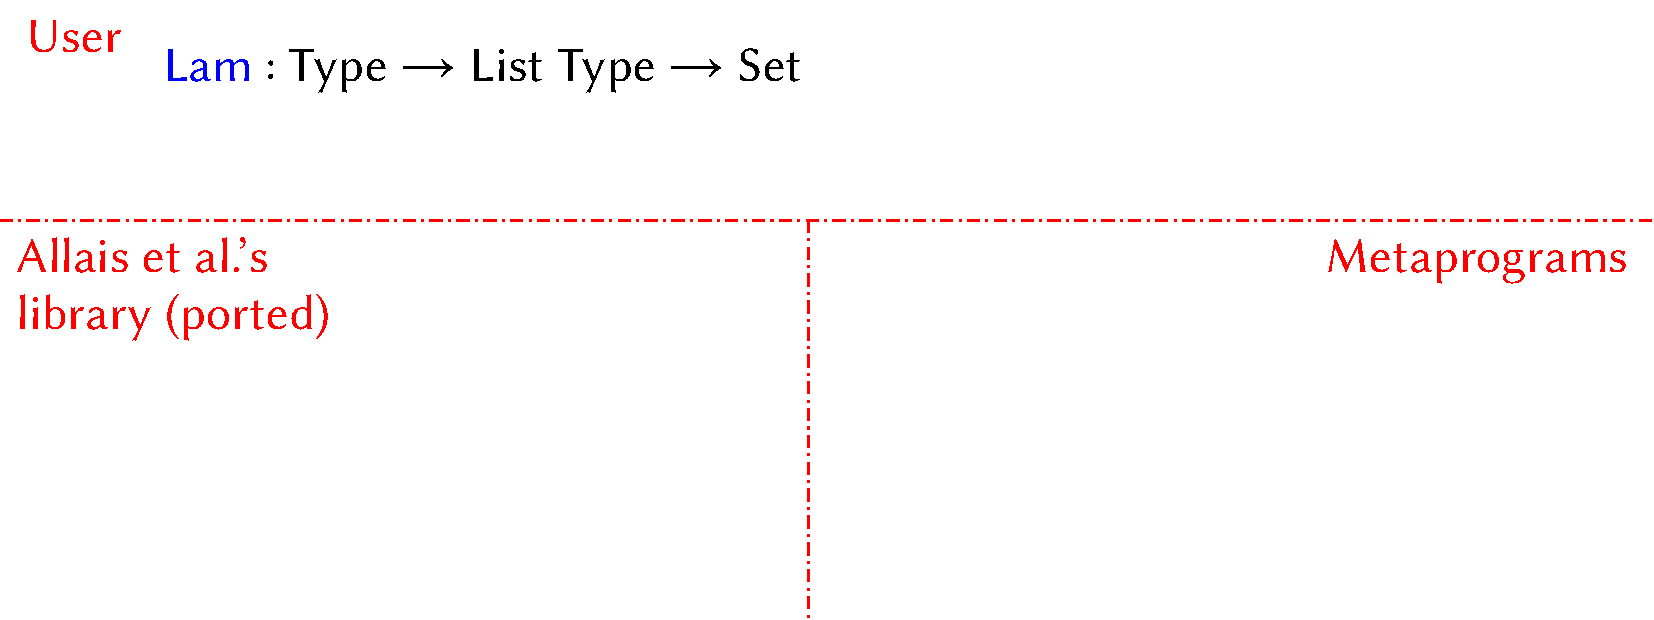
\includegraphics[width=\columnwidth]{Diagram1.pdf}
\end{frame}

\note{}

\begin{frame}[fragile]{Flow Chart}
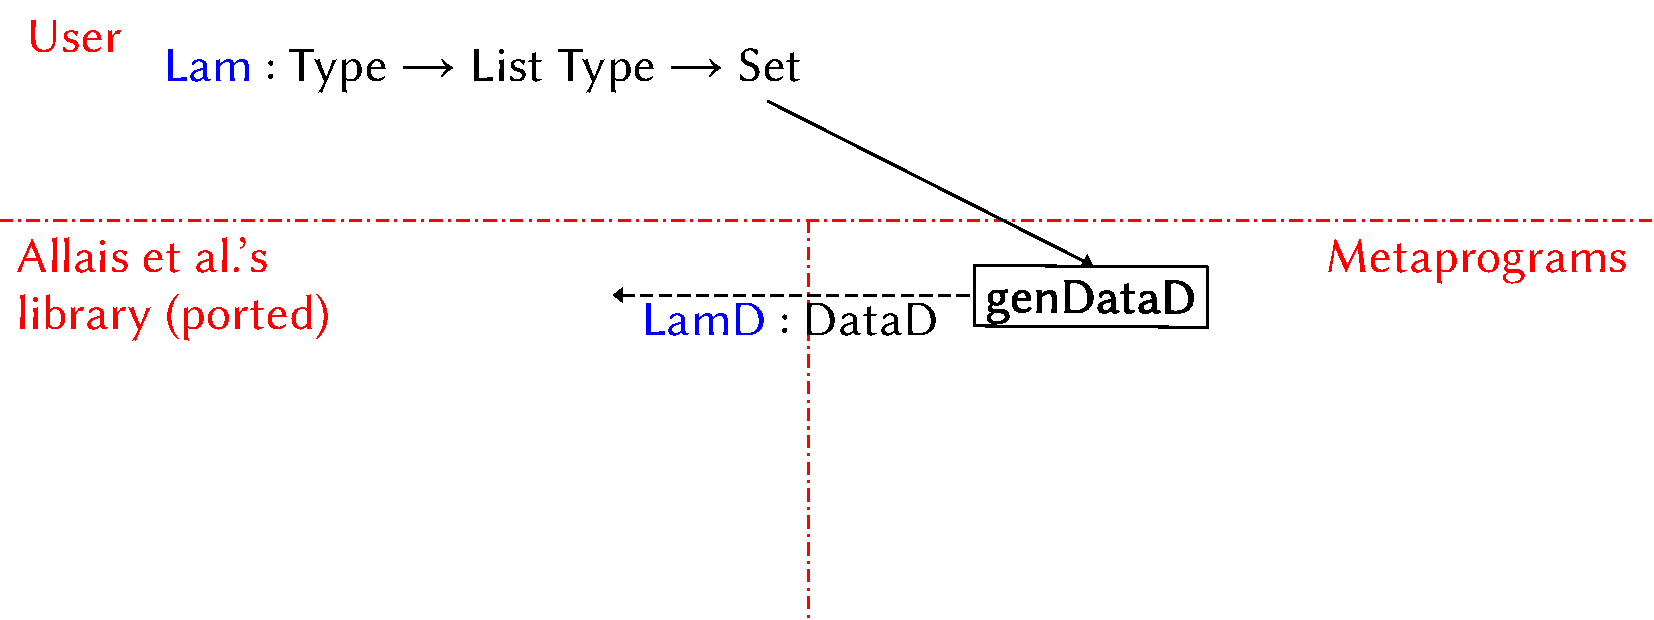
\includegraphics[width=\columnwidth]{Diagram2.pdf}
\end{frame}

\begin{frame}[fragile]{Flow Chart}
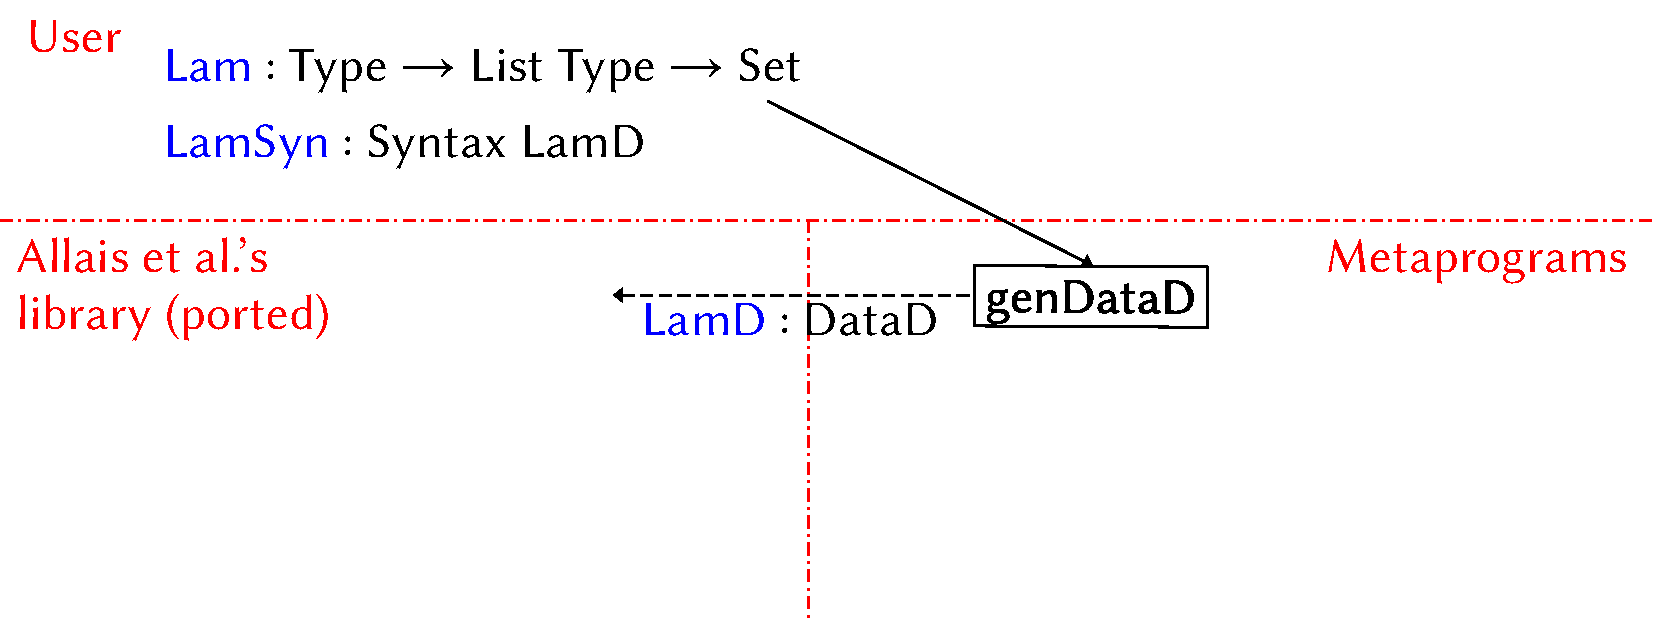
\includegraphics[width=\columnwidth]{Diagram3.pdf}
\end{frame}

\begin{frame}[fragile]{Flow Chart}
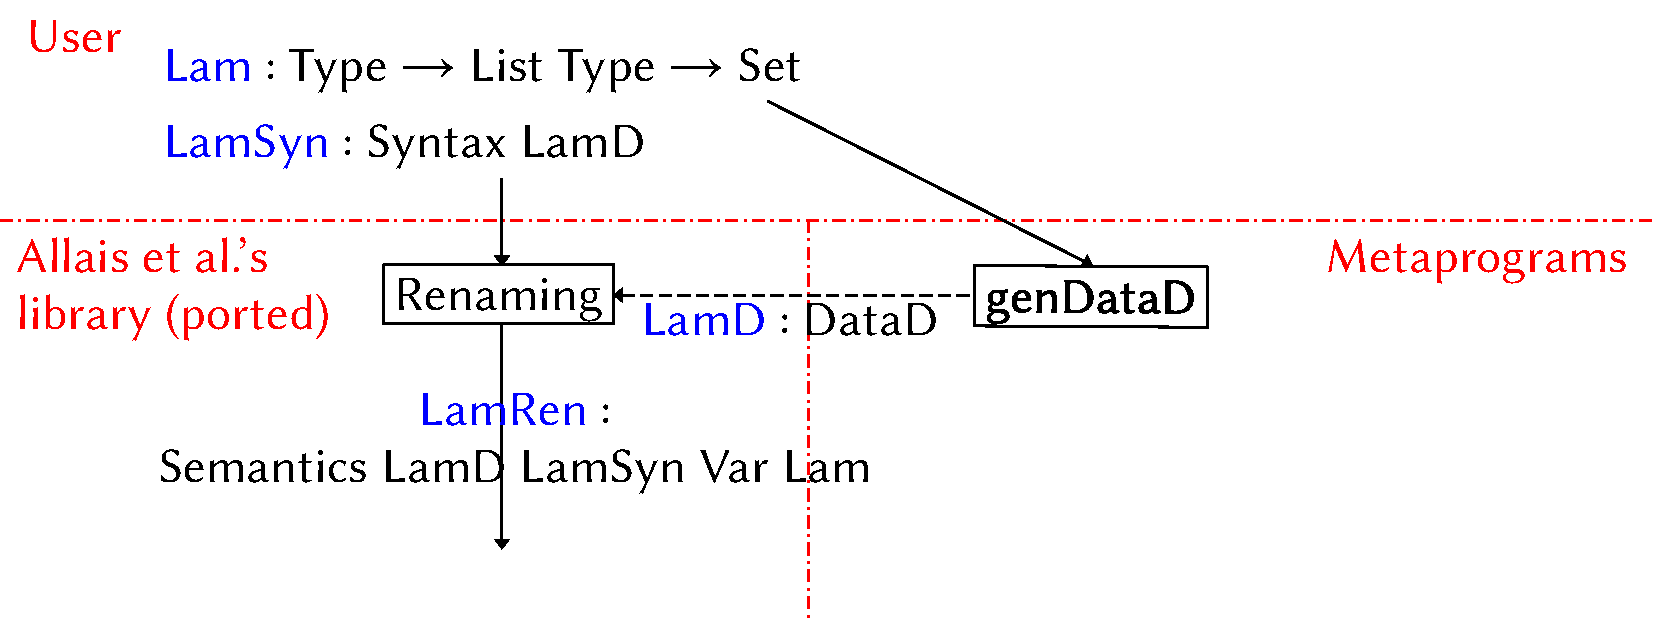
\includegraphics[width=\columnwidth]{Diagram4.pdf}
\end{frame}

\begin{frame}[fragile]{Flow Chart}
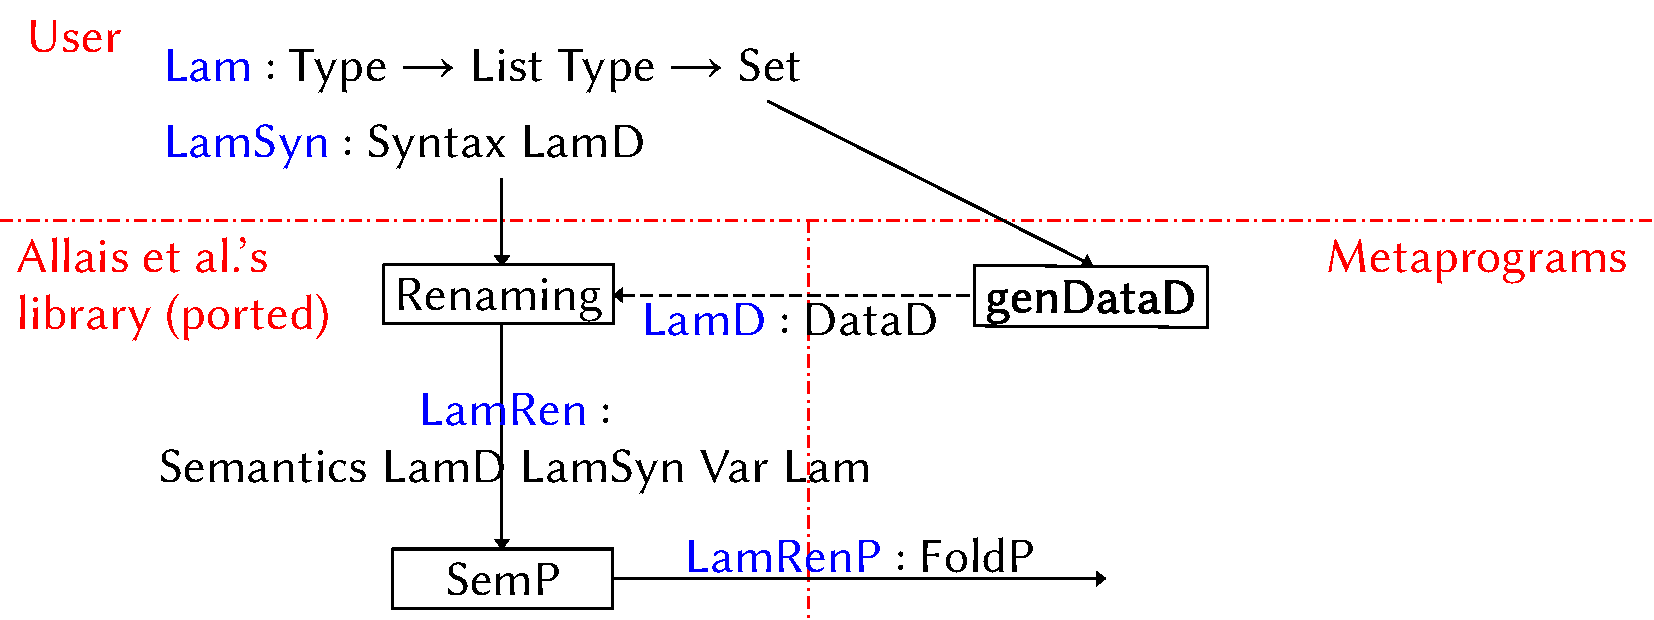
\includegraphics[width=\columnwidth]{Diagram5.pdf}
\end{frame}

\begin{frame}[fragile]{Flow Chart}
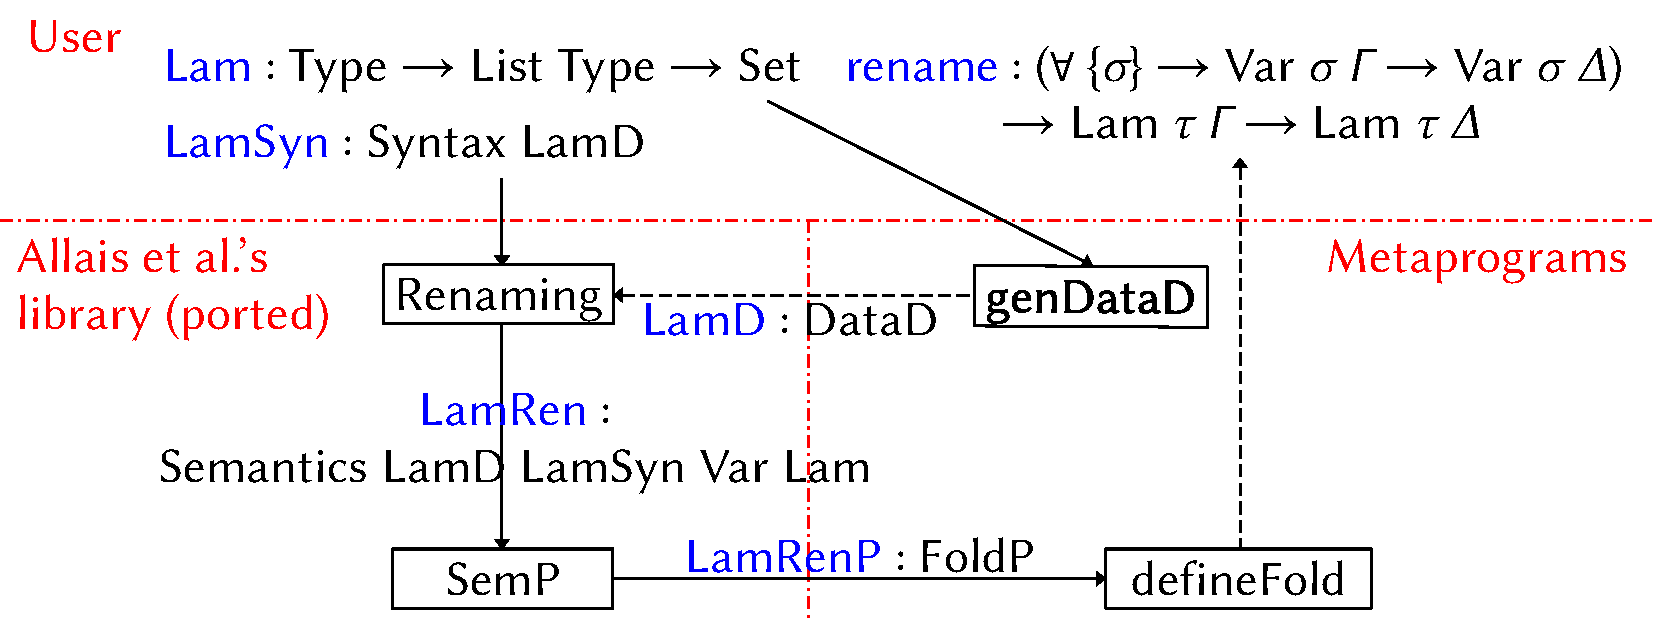
\includegraphics[width=\columnwidth]{Diagram6.pdf}
\end{frame}

\begin{frame}[fragile]{Provided by our datatype-generic library}
	\begin{itemize}
		\item a generic description \mi{DataD} for Agda's inductive datatypes,
		\pause
		\item generic program descriptions \mi{FoldP} for folds (and \mi{IndP} for inductions),
		\pause
		\item a metaprogram \mi{genDataD} that generates datatype descriptions from their native definitions, and 
		\pause
		\item a metaprogram \mi{defineFold} that generates function definitions from their generic representations.
	\end{itemize}
\end{frame}

\note{Here we introduce very berifly how we mixed datatype-generic programming with elaborator reflection. We have a generic description for all inductive datatypes and descriptions for generic programs, such }

\begin{frame}[fragile]{Elaborator Reflection to the Rescue}
	We further define:
	\begin{itemize}
		\item a predicate \mi{Syntax} on \mi{DataD} that captures \mi{Desc}.
		\item a function \mi{SemP} that generates \mi{FoldP} from \mi{Syntax} proofs.
	\end{itemize}
\end{frame}

\note{What does datatype-generic programming has to do with syntax-generic operations? We see that what the syntaxes programmers want are actually classic Agda inductive datatypes}


\begin{frame}[fragile]{The \mi{Syntax} Predicate}
	\begin{hscode}\SaveRestoreHook
\column{B}{@{}>{\hspre}l<{\hspost}@{}}%
\column{E}{@{}>{\hspre}l<{\hspost}@{}}%
\>[B]{}\Conid{Syntax}\;\mathbin{:}\;\Conid{Set}\;\Varid{ℓ}\;\Varid{→}\;\Conid{DataD}\;\Varid{→}\;\Conid{Setω}{}\<[E]%
\ColumnHook
\end{hscode}\resethooks
\mi{Desc} are captured by \mi{Syntax} as each:
	\pause
	\begin{itemize}
		\item has a variable rule,
		\pause
		\item is not universe polymorphic,
		\pause
		\item has two indices, $I$ and $\mi{List}\ I$, and
		\pause
		\item supports context extensions.
	\end{itemize}
\end{frame}

\begin{frame}[fragile]{The \mi{Syntax} Predicate}
Does \mi{PCF} satisfies \mi{Syntax}?
	\begin{hscode}\SaveRestoreHook
\column{B}{@{}>{\hspre}l<{\hspost}@{}}%
\column{3}{@{}>{\hspre}l<{\hspost}@{}}%
\column{10}{@{}>{\hspre}l<{\hspost}@{}}%
\column{27}{@{}>{\hspre}l<{\hspost}@{}}%
\column{E}{@{}>{\hspre}l<{\hspost}@{}}%
\>[B]{}\mathbf{data}\;\Conid{PCF}\;\mathbin{:}\;\Conid{Type}\;\Varid{→}\;\Conid{Context}\;\Varid{→}\;\Conid{Set}\;\mathbf{where}{}\<[E]%
\\
\>[B]{}\hsindent{3}{}\<[3]%
\>[3]{}\Varid{‵var}\;{}\<[10]%
\>[10]{}\mathbin{:}\;\Conid{Var}\;\Varid{σ}\;\Conid{Γ}\;\Varid{→}\;\Conid{PCF}\;\Varid{σ}\;\Conid{Γ}{}\<[E]%
\\
\>[B]{}\hsindent{3}{}\<[3]%
\>[3]{}\Varid{‵app}\;{}\<[10]%
\>[10]{}\mathbin{:}\;\Conid{PCF}\;(\Varid{σ}\;\Varid{⇒}\;\Varid{τ})\;\Conid{Γ}\;\Varid{→}\;\Conid{PCF}\;\Varid{σ}\;\Conid{Γ}\;\Varid{→}\;\Conid{PCF}\;\Varid{τ}\;\Conid{Γ}{}\<[E]%
\\
\>[B]{}\hsindent{3}{}\<[3]%
\>[3]{}\Varid{‵lam}\;{}\<[10]%
\>[10]{}\mathbin{:}\;\Conid{PCF}\;\Varid{τ}\;(\Varid{σ}\;\Varid{∷}\;\Conid{Γ})\;{}\<[27]%
\>[27]{}\Varid{→}\;\Conid{PCF}\;(\Varid{σ}\;\Varid{⇒}\;\Varid{τ})\;\Conid{Γ}{}\<[E]%
\\
\>[B]{}\hsindent{3}{}\<[3]%
\>[3]{}\Varid{‵zero}\;{}\<[10]%
\>[10]{}\mathbin{:}\;\Conid{PCF}\;\Varid{‵ℕ}\;\Conid{Γ}{}\<[E]%
\\
\>[B]{}\hsindent{3}{}\<[3]%
\>[3]{}\Varid{‵suc\char95 }\;{}\<[10]%
\>[10]{}\mathbin{:}\;\Conid{PCF}\;\Varid{‵ℕ}\;\Conid{Γ}\;\Varid{→}\;\Conid{PCF}\;\Varid{‵ℕ}\;\Conid{Γ}{}\<[E]%
\ColumnHook
\end{hscode}\resethooks
\end{frame}

\begin{frame}[fragile]{The \mi{Syntax} Predicate}
	\metroset{block=fill}
	\begin{exampleblock}{A Syntax proof example}
		\begin{hscode}\SaveRestoreHook
\column{B}{@{}>{\hspre}l<{\hspost}@{}}%
\column{9}{@{}>{\hspre}l<{\hspost}@{}}%
\column{E}{@{}>{\hspre}l<{\hspost}@{}}%
\>[B]{}\Conid{SyntaxPCF}\;\mathbin{:}\;\Conid{Syntax}\;\Conid{Type}\;(\Varid{genDataD}\;(\Varid{quote}\;\Conid{PCF})){}\<[E]%
\\
\>[B]{}\Conid{SyntaxPCF}\;\mathrel{=}\;\anonymous \;{}\<[E]%
\\
\>[B]{}\hsindent{9}{}\<[9]%
\>[9]{}\Varid{,}\;\Varid{refl}\;{}\<[E]%
\\
\>[B]{}\hsindent{9}{}\<[9]%
\>[9]{}\Varid{,}\;(\Varid{refl}\;\Varid{,refl})\;{}\<[E]%
\\
\>[B]{}\hsindent{9}{}\<[9]%
\>[9]{}\Varid{,}\;\anonymous \;{}\<[E]%
\\
\>[B]{}\hsindent{9}{}\<[9]%
\>[9]{}\Varid{,}\;\Varid{refl}\;{}\<[E]%
\\
\>[B]{}\hsindent{9}{}\<[9]%
\>[9]{}\Varid{,}\;\Varid{refl}\;{}\<[E]%
\\
\>[B]{}\hsindent{9}{}\<[9]%
\>[9]{}\Varid{,}\;(\anonymous \;\Varid{,}\;\anonymous \;\Varid{,}\;\anonymous \;\Varid{,}\;\Varid{refl}\;\Varid{,}\;(\Varid{λ}\;\anonymous \;\Varid{→}\;\Varid{refl}))\;{}\<[E]%
\\
\>[B]{}\hsindent{9}{}\<[9]%
\>[9]{}\Varid{,}\;(\anonymous \;\Varid{,}\;\anonymous \;\Varid{,}\;\anonymous \;\Varid{,}\;\Varid{refl}\;\Varid{,}\;(\Varid{λ}\;\anonymous \;\Varid{→}\;\Varid{refl}))\;{}\<[E]%
\\
\>[B]{}\hsindent{9}{}\<[9]%
\>[9]{}\Varid{,}\;(\anonymous \;\Varid{,}\;\anonymous \;\Varid{,}\;\anonymous \;\Varid{,}\;\Varid{refl}\;\Varid{,}\;(\Varid{λ}\;\anonymous \;\Varid{→}\;\Varid{refl}))\;{}\<[E]%
\\
\>[B]{}\hsindent{9}{}\<[9]%
\>[9]{}\Varid{,}\;(\anonymous \;\Varid{,}\;\anonymous \;\Varid{,}\;\anonymous \;\Varid{,}\;\Varid{refl}\;\Varid{,}\;(\Varid{λ}\;\anonymous \;\Varid{→}\;\Varid{refl}))\;{}\<[E]%
\\
\>[B]{}\hsindent{9}{}\<[9]%
\>[9]{}\Varid{,}\;\Varid{tt}{}\<[E]%
\ColumnHook
\end{hscode}\resethooks
	\end{exampleblock}
\end{frame}

% \begin{frame}[fragile]{Translation from Semantics to natural looking functions}
% \end{frame}

\section{Demo}

\section{Discussion: towards datatype-generic libraries for syntaxes?}

\begin{frame}[fragile]{Future Works \& Issues}
	\begin{itemize}
		\item \mi{Syntax} proof automation
		\item User interface
		\item Port more generic libraries:
		\pause
			\begin{itemize}
				% \item Expressiveness is limited by Agda datatypes as well as the generic universe, a \mi{Syntax} predicate must be defined.
				% \pause
				% \item Even if we can define \mi{Syntax}, the proof could be more complicated, even require programmers to understand the generic universe.
				% \pause
				% \item Obstacles of using multiple generic libraries at once.
				% \pause
				% \item Are folds and inductions enough?
				\item Expressiveness
				\pause
				\item Complexity of \mi{Syntax}
				\pause
				\item Interoperability
				\pause
				\item Are folds and inductions enough?
			\end{itemize}
	\pause
	\end{itemize}
\end{frame}

\section{Q \& A}

\end{document}

